%TODO The caption and the image are from http://swarmlab.unimaas.nl/stico/stico-principle/ so there needs to be a reference to here
\cite{ranjbar2012multi}
\begin{figure}[htp!]
\centering
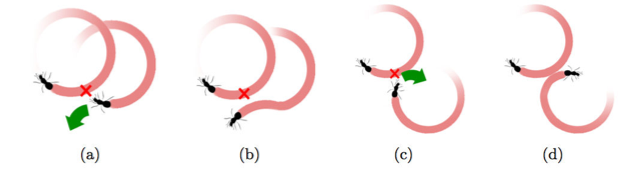
\includegraphics[width=\columnwidth]{images/stico.png}
\caption{StiCo coordination principle (a) and (c) before pheromone detection (b) and (d) after pheromone detection}
\label{fig:overall}
\end{figure}

Take the movement ruels of StiCo

the same concept as the following text applies but the difference is is that we dont look to the pherome but use the vision to determn the movement derection 

% the source of this text is http://swarmlab.unimaas.nl/stico/stico-principle/
When the interior sensor detects pheromone (i.e. the trails on the floor), it means that the robot is entering another territory, so the robot changes circling direction immediately as shown in Figures 1a, and 1b. Otherwise, if exterior sensor detects pheromone, it means that the robot is passing near another territory, so the robot rotates in the same direction (i.e. angular speed is increased temporary) until it doesn’t detect pheromone any more, and then circles in the same direction with the previous constant angular velocity as shown in 